\documentclass{beamer}
\usepackage{graphicx}
\usepackage{graphics}
\usepackage{hyperref}
\usepackage[english]{babel}


\mode<presentation>
{
    \usetheme{AMUFree-kk}
    \setbeamercovered{transparent = 28}
}
\title{Focused Hierarchical RNNs}
\date{2018}
\author{Karol Kaczmarek}
\setbeamertemplate{bibliography item}{[\theenumiv]}

\begin{document}

\begin{frame}
    \titlepage
\end{frame}


% The upper states of our network can be considered as a memory focusing on relevant information that can be attended to at each step of the answer generation process.

\section{Ideas}

\begin{frame}
    \frametitle{Ideas}
    \begin{itemize}
        \item reading a Wikipedia article and trying to identify information that is relevant to answering a question
        \begin{itemize}
            \item before one knows what the question is
            \item where context or question is given before reading the article
        \end{itemize}
    \end{itemize}
\end{frame}


\section{Architecture}

\begin{frame}
    \frametitle{Architecture}
    \begin{itemize}
        \item Focused Hierarchical RNNs for Conditional Sequence Processing \cite{focused_hierarchical_rnns}
        \begin{itemize}
            \item focused hierarchical encoder (FHE)
            %\item context encoder
            \item decoder
        \end{itemize}
        \item Focused Hierarchical Encoder = two-layer LSTM
        \begin{itemize}
            \item lower layer operates at the input token level
            \item upper layer focuses on tokens relevant to the context
            \item conditional boundary gate to decide, depending on the context or question whether it is useful to update the upper-level LSTM
        \end{itemize}
    \end{itemize}
\end{frame}

\begin{frame}
    \frametitle{Focused Hierarchical Encoder - visualization}

    \begin{center}
        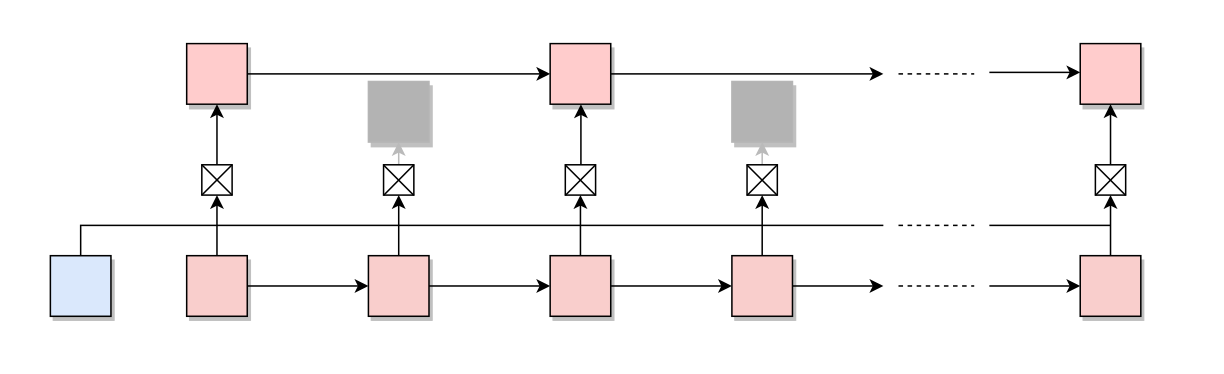
\includegraphics[scale=0.9]{img/FHE.png}
    \end{center}
    \begin{itemize}
        \item lower layer LSTM processes each step
        \item for each token, the boundary gate decides (based on the current lower layer LSTM state and question embedding) if information should be stored in the upper level
        \item higher layer LSTM states update only when the corresponding gate is open
    \end{itemize}
\end{frame}

\begin{frame}
    \frametitle{Lower-level Layer}
    \begin{itemize}
        \item $ h_t^l, c_t^l = $ LSTM$(x_t, h_{t-1}^l, c_{t-1}^l) $
        \item sequence of input tokens - $ P = (x_1, ..., x_n) $
        \item LSTM hidden state - $ h_t^l $
        \item LSTM cell state - $ c_t^l $
        \item time - $ t $
        \item may be also augmented with other available information (question encoding)
    \end{itemize}
\end{frame}

\begin{frame}
    \frametitle{Conditional Boundary Gate}
    \begin{itemize}
        \item decides if information at the current time step should be stored in the upper-level representation
        \item question is essential in deciding how to represent the passage
        \item question embedding - $ q $
        \item output of the boundary gate is a scalar $ b_t \in (0,1) $ that
is taken to be the parameter of a Bernoulli distribution $ b_t \sim $ Bernoulli$(b_t)$
        \item time - $ t $
    \end{itemize}
\end{frame}

\begin{frame}
    \frametitle{Conditional Boundary Gate}
    \begin{itemize}
        \item in the simplest case, the boundary gate forward pass is
formulated as $ \tilde{b}_t = \sigma(w_b^{\top}$LReLU$(W_b z_t + b_b)) $
        \item trainable weights - $ W_b, b_b, w_b $
        \item leaky ReLU - LReLU$(x) = \left\{
        \begin{array}{ll}
        x & \textrm{if } x>0 \\
        0.01x & \textrm{otherwise}
        \end{array} \right. $
        \item input - $ z_t = [q \odot h_t^l, h_t^l, q] $
        \item element-wise product - $ \odot $
        \item lower-layer hidden states - $ h_t^l $
        \item question embedding - $ q $
    \end{itemize}
\end{frame}

\begin{frame}
    \frametitle{Upper-level Layer}
    \begin{itemize}
        \item $ \tilde{h}_t^u, \tilde{c}_t^u = $ LSTM$(h_t^l, h_{t-1}^u, c_{t-1}^u) $
        \item $ b_t \sim $ Bernoulli$(b_t)$
        \item $ c_t^u = \tilde{b}_{t}\tilde{c}_t^u + (1 - \tilde{b}_{t})c_{t-1}^u $
        \item $ h_t^u = \tilde{b}_{t}\tilde{h}_t^u + (1 - \tilde{b}_{t})h_{t-1}^u $
        \item LSTM hidden state - $ h_t^u $
        \item LSTM cell state - $ c_t^u $
        \item time - $ t $
    \end{itemize}
\end{frame}


\section{Experiments}

\begin{frame}
    \frametitle{Baseline}
    \begin{itemize}
        \item LSTM1 (1-layer LSTM) - equivalent to FHE with the always closed ($b_t = 0$ for each $t$)
        \item LSTM2 (2-layer LSTM) - equivalent to FHE with the boundary gate fully open ($b_t = 1$ for each $t$)
    \end{itemize}
\end{frame}

\begin{frame}
    \frametitle{Picking task}
    \begin{itemize}
        \item given a sequence of randomly generated digits of length $n$
        \item the goal is to determine the most frequent digit within the first $k$ digits ($k \le n$)
        \item where value $k$ is the question
        \item tested for $n \in \{100, 200, 400\}$
    \end{itemize}
\end{frame}

\begin{frame}
    \frametitle{Picking task - examples}
    \begin{center}
        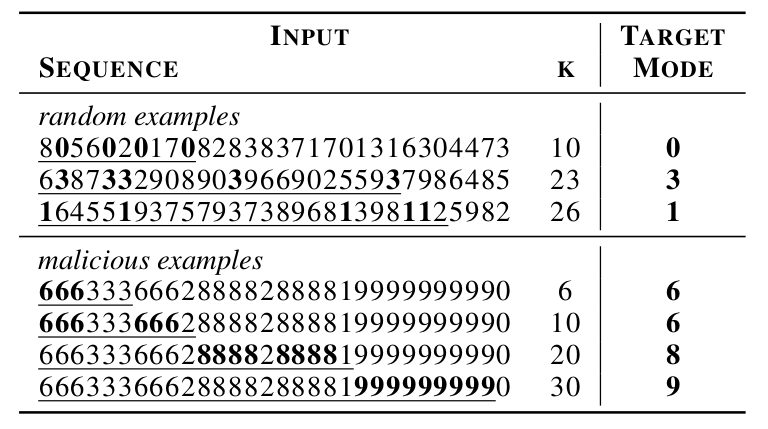
\includegraphics[scale=1.5]{img/picking-table1.png}
    \end{center}
\end{frame}

\begin{frame}
    \frametitle{Picking task - hyper-parameters}
    \begin{itemize}
        \item hidden $= 128$, learning rates $=  0.0001$, Adam optimizer
        \item fix hyper-parameters to a small value (for examples $\beta = 0.1$ and $\gamma = 0.25$) - gates can almost freely open
        \begin{itemize}
            \item once the desired accuracy has been reached, enforce constraints on our hyper-parameters
            \item provides a level of control over the accuracy-sparsity tradeoff
            \item this approach with the requirement of achieving a desired accuracy $a \in \{80\%, 90\%, 95\%, 98\%\}$, called: FHE80, FHE90, FHE95, FHE98
        \end{itemize}
        \item fix hyper-parameters more restricted than previous (for examples $\beta = 1$ and $\gamma = 0.1$), called FHE-fixed
    \end{itemize}
\end{frame}

\begin{frame}
    \frametitle{Picking task - results}
    \begin{center}
        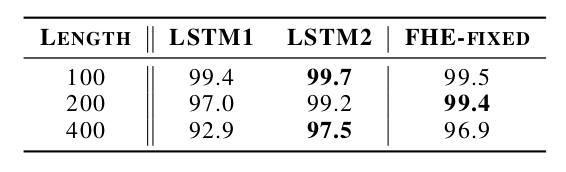
\includegraphics[scale=1.8]{img/picking-table2.png}
        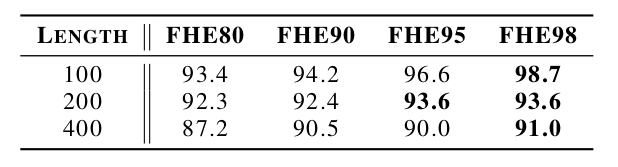
\includegraphics[scale=1.8]{img/picking-table3.png}
    \end{center}
\end{frame}

\begin{frame}
    \frametitle{Picking task - test for longer sequence length}
    \begin{itemize}
        \item models trained on short sequences ($n=200$)
        \item evaluated on longer sequences and $k \le 200$
    \end{itemize}
    \begin{center}
        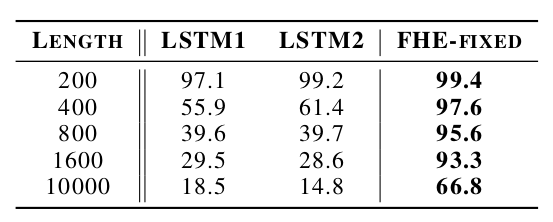
\includegraphics[scale=1.8]{img/picking-table4.png}
    \end{center}
\end{frame}

\begin{frame}
    \frametitle{Pixel-by-Pixel MNIST QA task}
    \begin{itemize}
        \item adapt the Pixel-by-Pixel MNIST classification task to the question and answering setting
        \item encoder reads in MNIST digits one pixel at a time
        \item question asked is whether the image is a specific digit and the answer is either True or False
    \end{itemize}

    \begin{center}
        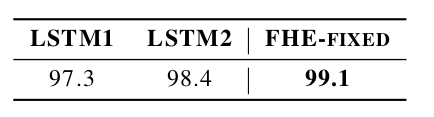
\includegraphics[scale=1.8]{img/digits-table.png}
    \end{center}
\end{frame}

\begin{frame}
    \frametitle{Pixel-by-Pixel MNIST QA task}
    \begin{itemize}
        \item model learns to open the boundary gate almost always around the digit
        \item gates do not depend on the question
    \end{itemize}

    \begin{center}
        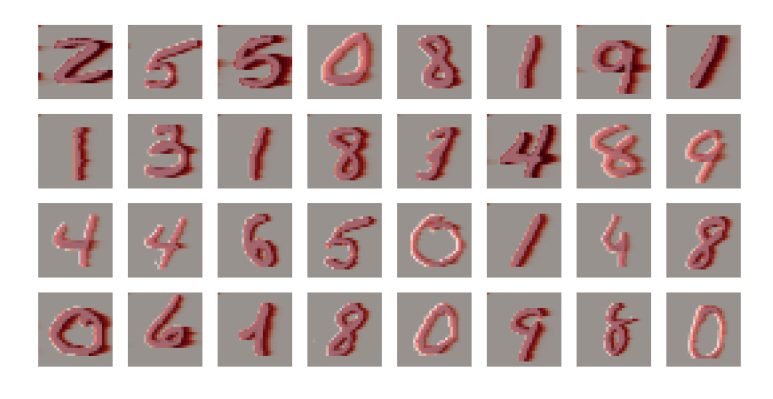
\includegraphics[scale=1.6]{img/digits.png}
    \end{center}
\end{frame}

\begin{frame}
    \frametitle{Natural Language QA Tasks}
    \begin{itemize}
        \item using the MS MARCO and SearchQA datasets and tasks
        \item use a bidirectional LSTM for question
        \item hidden $= 300$, learning rate $= 0.001$, Adam optimizer
        \item to avoid large-vocabulary issues, use the pointer softmax
        \begin{itemize}
            \item distribution over a shortlist of words ($100, 10000$ most frequent words for SearchQA or MS MARCO tasks) - $o_j$
            \item distribution over words in the document - $x_j$
            \item variable $z_j$ determines how to interpolate between the indices in the document and the shortlist words
            \item $P_j = [z_{j}o_{j};(1-z_j)\alpha_j]$
        \end{itemize}
    \end{itemize}
\end{frame}

\begin{frame}
    \frametitle{SearchQA Question and Answering Task}
    \begin{itemize}
        \item large scale QA dataset in the form of Question-Context-Answer
        \item question-answer pairs are real Jeopardy! (crawled from
J!Archive)
        \item contexts are text snippets retrieved by Google
        \item use F1 scores for multi-word answers
        \item use Exact Match (EM) for single word answers
    \end{itemize}
\end{frame}

\begin{frame}
    \frametitle{SearchQA Question and Answering Task - results}
    \begin{center}
        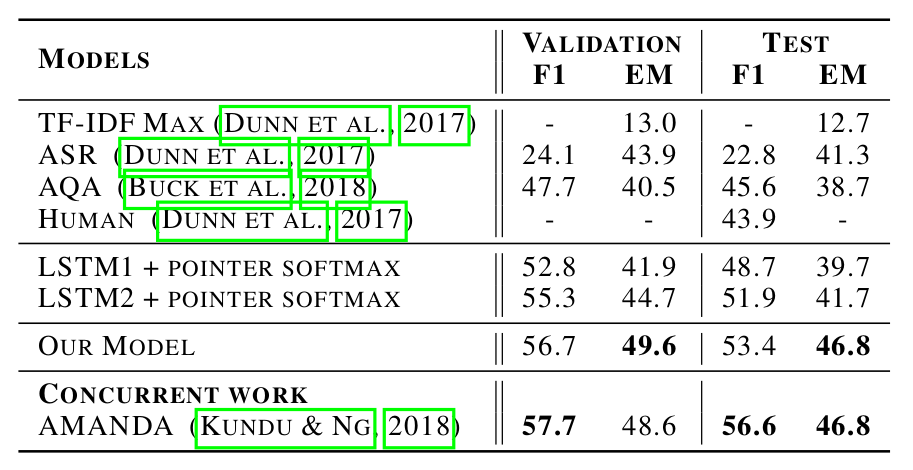
\includegraphics[scale=1.45]{img/searchqa-table.png}
    \end{center}
\end{frame}

\begin{frame}
    \frametitle{MS MARCO Question and Answering Task}
    \begin{itemize}
        \item one of the largest publicly available QA datasets
        \item example in the dataset consists of a query
        \item several context passages retrieved by the Bing search engine
        \item several human generated answers (synthesized from the given contexts)
        \item contains many rare words, with around 90\% of words appealing less than 20 times in the dataset
    \end{itemize}
\end{frame}

\begin{frame}
    \frametitle{MS MARCO Question and Answering Task}
    \begin{itemize}
        \item span-based
        \begin{itemize}
            \item state of the art according to Bleu-1 and Rouge scores
            \item trained using "gold-spans", obtained by a preprocessing step which selects the passage in the document maximizing the Bleu-1 score with the answer
            \item they cannot answer questions where the answer is not contained in the passage
        \end{itemize}
        \item generative systems
        \begin{itemize}
            \item synthesize a novel answer for the given question
            \item could learn a disentangled representation, and therefore generalize better
        \end{itemize}
    \end{itemize}
\end{frame}

\begin{frame}
    \frametitle{MS MARCO Question and Answering Task - span-based systems}
    \begin{itemize}
        \item state of the art according to Bleu-1 and Rouge scores
        \item trained using "gold-spans", obtained by a preprocessing step which selects the passage in the document maximizing the Bleu-1 score with the answer
        \item they cannot answer questions where the answer is not contained in the passage
    \end{itemize}
\end{frame}

\begin{frame}
    \frametitle{MS MARCO Question and Answering Task - results}
    \begin{center}
        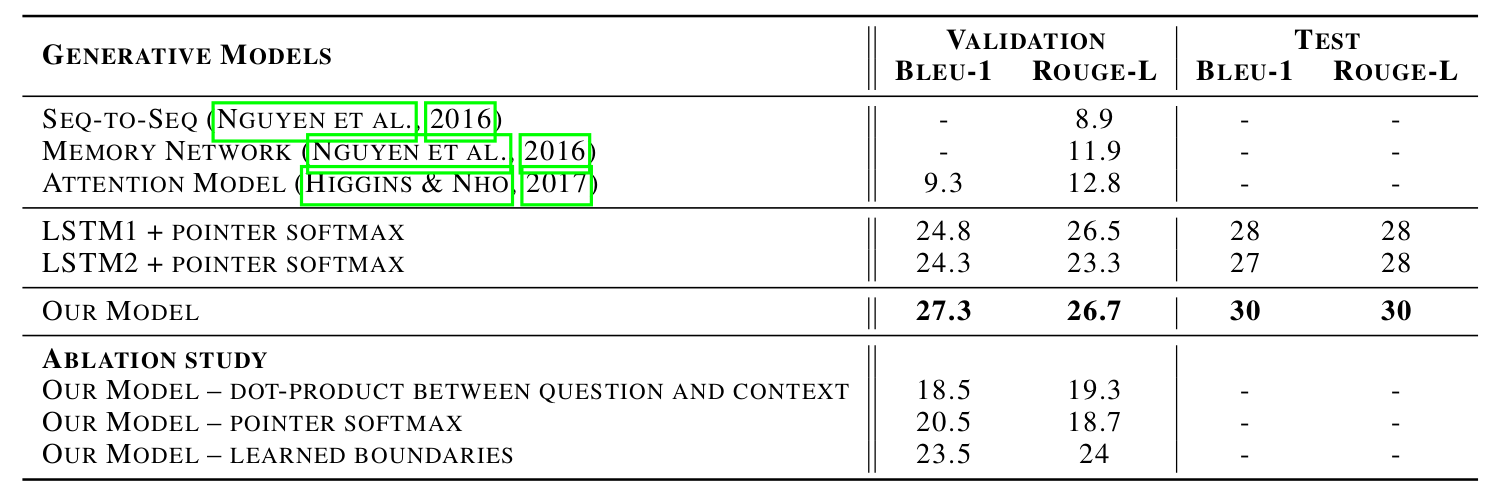
\includegraphics[scale=0.9]{img/msmarco-table.png}
    \end{center}
\end{frame}


% References
\section{References}
\begin{frame}[allowframebreaks,t]
    \tiny
    \frametitle{References}
    \bibliographystyle{ieeetr}
    \bibliography{focused_hierarchical_rnns}
    %\nocite{*}
\end{frame}

\end{document}
